% !TEX root =  master.tex
\chapter{Präsentation der PWA}
In diesem Kapitel wird die umgesetzte PWA, die zuvor durch Mockups dargestellt wurde, vorgestellt. Da die Grundlagen zur Technologie bereits im Kapitel 3 ausführlich erläutert worden sind, wird hier nicht mehr näher auf die Implementierungsdetails eingegangen,
sondern lediglich das Resultat anhand von Screenshots vorgestellt. Abschließend findet noch ein Abgleich mit den zuvor definierten Anforderungen statt.

Die Umsetzung der PWA erfolgte mithilfe der JavaScript-
Bibliothek React auf Basis des entwickelten Prototypen. Im Folgenden wird der aktuelle Entwicklungsstand
der App näher vorgestellt. Dabei wird auf die Gestaltung
und die Navigation als auch auf die Funktionalität der PWA eingegangen.

\begin{figure}[h!]
	\centering
	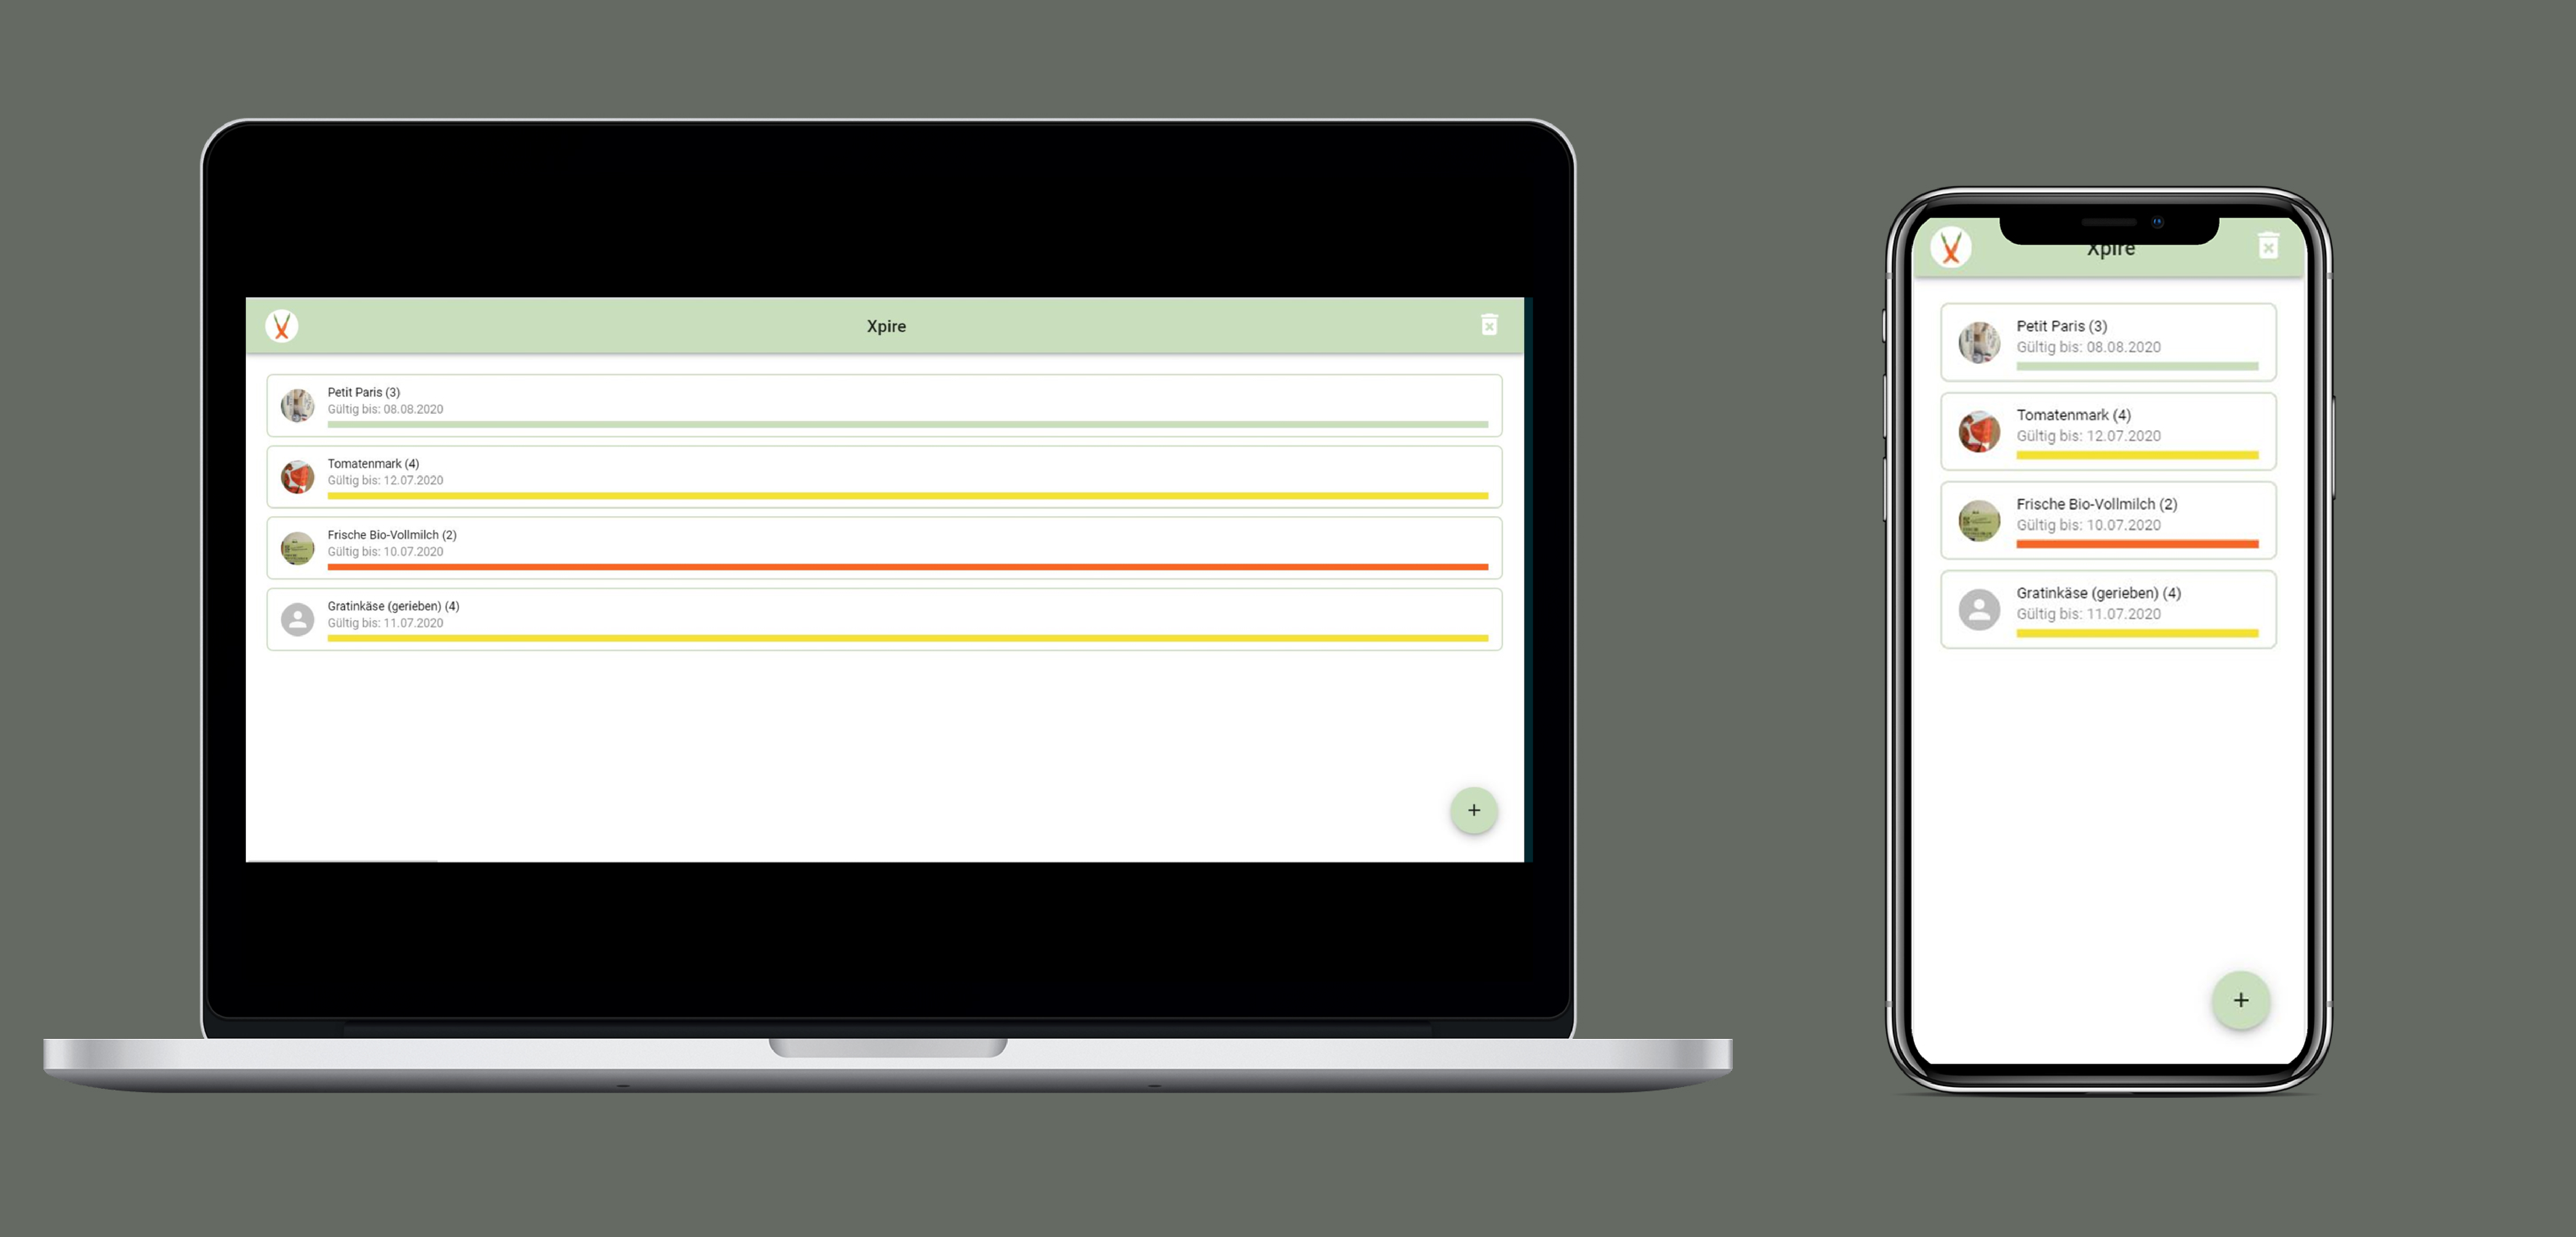
\includegraphics[width=1.0\textwidth]{img/app.pdf}
	\caption{Xpire auf Laptop vs. Smartphone}
	\label{fig:app}
\end{figure}

%\begin{wrapfigure}{r}{0.5\textwidth}
%	\vspace{-1.5\baselineskip}
%	\begin{center}
%		
\includegraphics[width=0.50\textwidth]{img/plus.jpg}
%	\end{center}
%	\setcapindent{0cm}
%	\caption{Ausschnitt des ungerichteten Graphen zum %Einkauf-Problem}
%	\label{fig:graph_edeka}
%\end{wrapfigure}

Die Abbildung \ref{fig:app} zeigt, wie sich die Xpire-App verschiedenen Bildschirmgrößen problemlos anpasst. Zu sehen ist der \textit{Home-Screen} mit einer Auswahl an Beispiel-Produkten sowohl auf dem Laptop als auch auf dem Smartphone.\\
Um Xpire auf dem Laptop zu installieren, muss man folgenden Link in die Adresszeile seines Browsers eingeben: https://felixwaage.github.io/Xpire/. Es erscheint die App,  wie zu sehen in Abbildung \ref{fig:install} im Browser und lässt sich über ein "+" ganz rechts in der Adresszeile als App dem Desktop hinzufügen. Nach einem Klick auf den Plus-Button öffnet sich ein Pop-Up, welches es dem Nutzer ermöglicht, die Installation durchzuführen. Klick man den Installations-Button, wird im dritten Schritt die Xpire-App auf dem Desktop hinterlegt, siehe \ref{fig:install}.

\begin{figure}[h!]
	\centering
	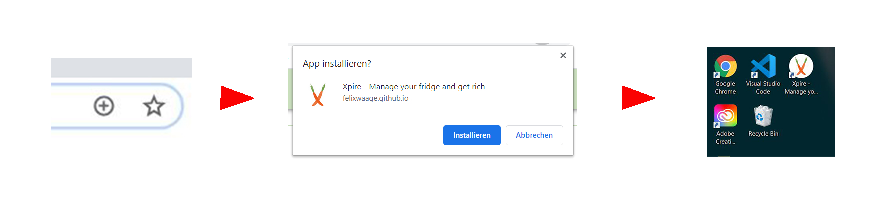
\includegraphics[width=1.1\textwidth]{img/install.pdf}
	\caption{Xpire-Installationsprozess am Laptop}
	\label{fig:install}
\end{figure}

Die Installation auf dem Smartphone erfolgt äquivalent zu der auf dem Desktop. Nach dem Öffnen des Links wid über ein Pop-Up die Möglichkeit zur Installation bereit gestellt. Xpire wird dann auf dem Smartphone angezeigt wie eine native mobile App und weist auch nach dem Öffnen keine Unterschiede zu einer nativen App auf. Dennoch läuft die App als PWA komplett im Browser. 

Damit die User Experience der PWA-Applikation auf dem Smartphone ähnlich zu einer nativen Applikation ist, wird ein sogenannter Splash Screen implementiert. Dieser erscheint nachdem der Benutzer die auf dem Smartphone gespeicherte Xprie-PWA öffnet. In Abbildung \vref{fig:splashScreen} werden die Splash Screens abgebildet, wobei dieser bei einem iOS-Betriebssysteme in weiß und für Android-Geräte in grün erscheint.  

Der Splash Screen sowie weitere Funktionalität der Xpire-Applikation sind in einer Bildschirmaufnahme mit dem Betriebssystem iOS zu sehen, welche unter folgendem Link verfügbar ist:\\
\url{https://github.com/felixwaage/Xpire/blob/master/iOS-Bildschirmaufnahme.mov} 

\begin{figure}[H]
	\centering
	\subfigure[iOS]{
\includegraphics[width=0.30\textwidth]{img/splashScreenIos.png}} 
	\subfigure[Android]{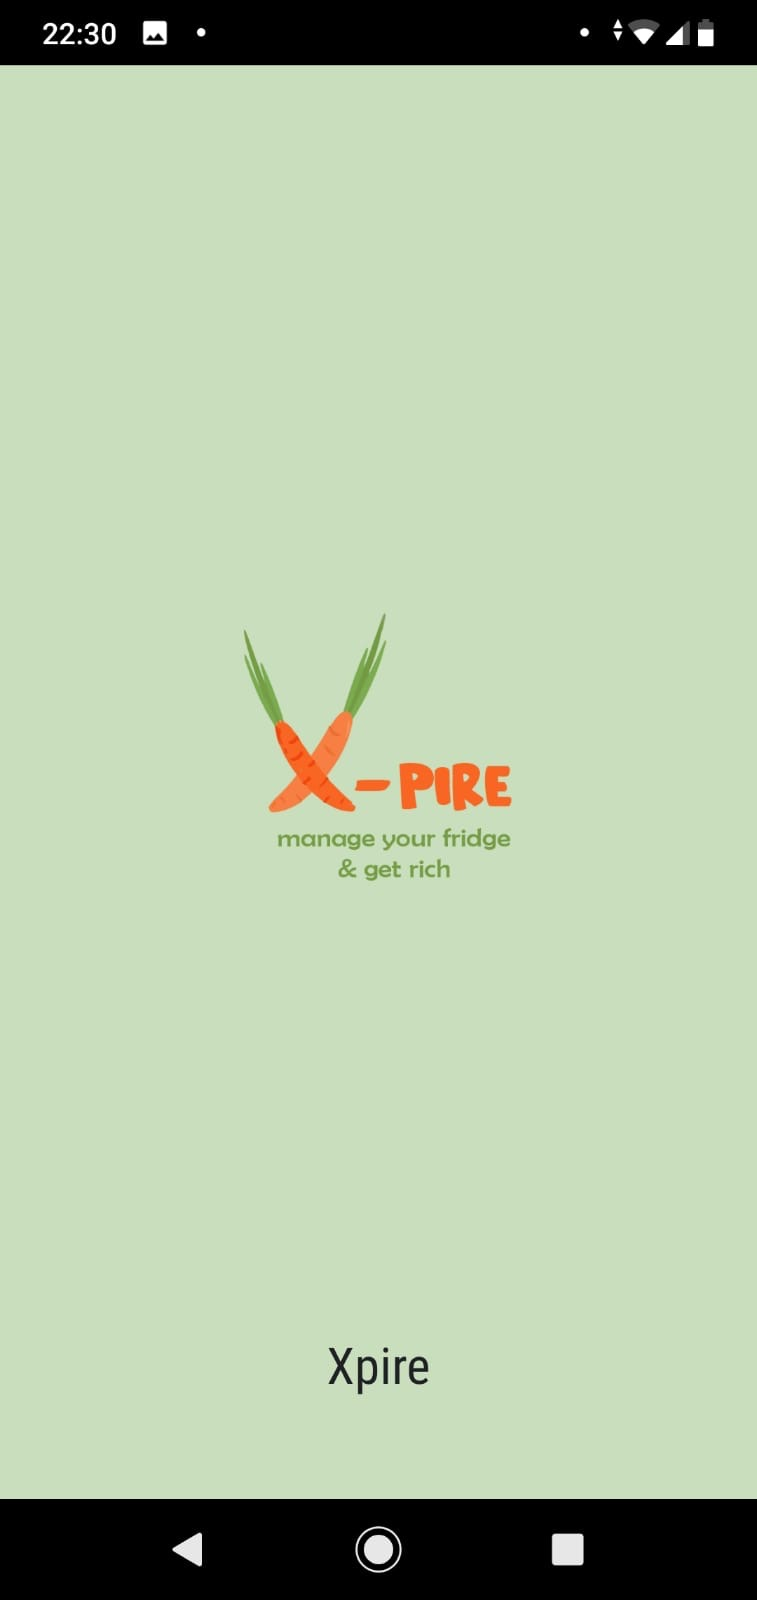
\includegraphics[width=0.30\textwidth]{img/splashScreenAndroid.jpg}} 
	\caption{Splash Screen für iOS und Android}
	\label{fig:splashScreen}
\end{figure}

% was ist unterschiedlich im Vergleich zu den Mockups?
Die Gestaltung als auch der User-Flow der entwickelten PWA entsprechen fast eins zu eins dem der Mockups. Geringe Unterschiede lassen sich an folgenden Punkten feststellen:
 \begin{itemize}[noitemsep]
 	\item \textbf{AppBar:} Das Logo in der entwickelten PWA hat einen weißen Kreis als Hintergrund. Das Icon oben recht ist nicht wie im Mockup ein Zahnrad, sondern ein weißes Mülleimer-Icon.
 	\item \textbf{Produkt löschen:} Die Produkte lassen sich einzeln nicht direkt im \textit{Home-Screen} per Wischen nach links, wie designed im Mockup, löschen, sondern lediglich im \textit{Produkt-Screen} über ein Mülleimer-Icon. Wird jedoch das Mülleimer-Icon oben rechts in der AppBar des \textit{Home-Screen} dar, erhält der Nutzer die Möglichkeit, alle hinterlegten Produkte auf einmal zu löschen.
 	\item \textbf{Produkte verwalten:} Der \textit{Produkt-Screen} wurde implementiert, so wie er im Mockup designed wurde. Das hinterlegte Bild wird angezeigt und Name, Anzahl, Einkaufsdatum und Ablaufdatum lassen sich durch das Anklicken des jeweiligen Textfeldes ändern. Lediglich die Terminologie des Buttons hat wurde von \enquote{Speichern} zu \enquote{Ändern} verändert.
 \end{itemize}

%neuer Screen: Produkt hinzufügen 
Neben der Umsetzung des erstellten Mockups, wurde zusätzlich eine Ansicht zum Hinzufügen eines neuen Produktes entwickelt, zu sehen in Abbildung \ref{fig:add}. Der Nutzer hat die Möglichkeit einen Barcode zu scannen oder ihn manuell im Barcode-Textfeld einzugeben. Über die OpenFood-API wird automatisch das jeweilige Produktbild angezeigt und der Titel im dazugehörigen Feld angezeigt.

\begin{figure}[h!]
	\centering
	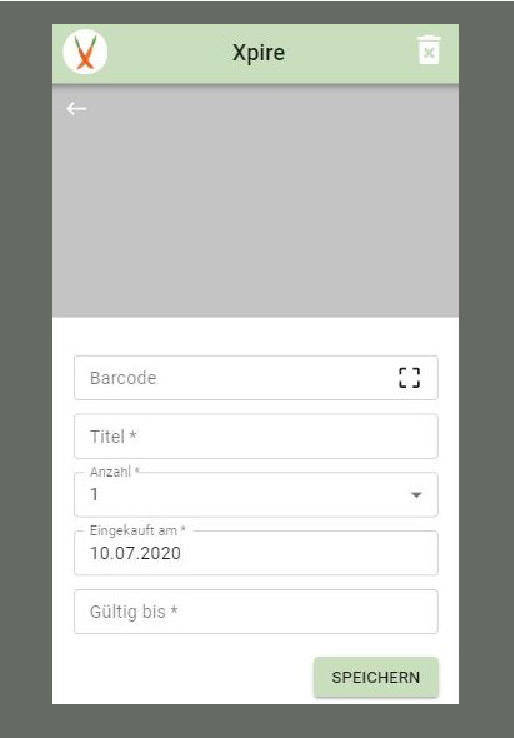
\includegraphics[width=0.6\textwidth]{img/add.pdf}
	\caption{Produkt hinzufügen}
	\label{fig:add}
\end{figure}

Die Standard-Anzahl der Produkte beträgt 1, lässt sich aber über ein Dropdown einfach erhöhen. In dem Eingabefeld für das Einkaufsdatum ist automatisch das aktuelle Datum vorausgewählt, was sich jedoch ändern lässt, sobald man in das Textfeld reinklickt. Es öffnet sich ein Date-Picker, genau wie bei der Eingabe des Gültigkeitsdatums. Nach dem Speichern wird das Produkt automatisch dem \textit{Home-Screen} hinzugefügt.


% Tests --> feingarnulare Unit Tests, acceptance tests?

